\documentclass{standalone}
\usepackage{tikz}

\begin{document}

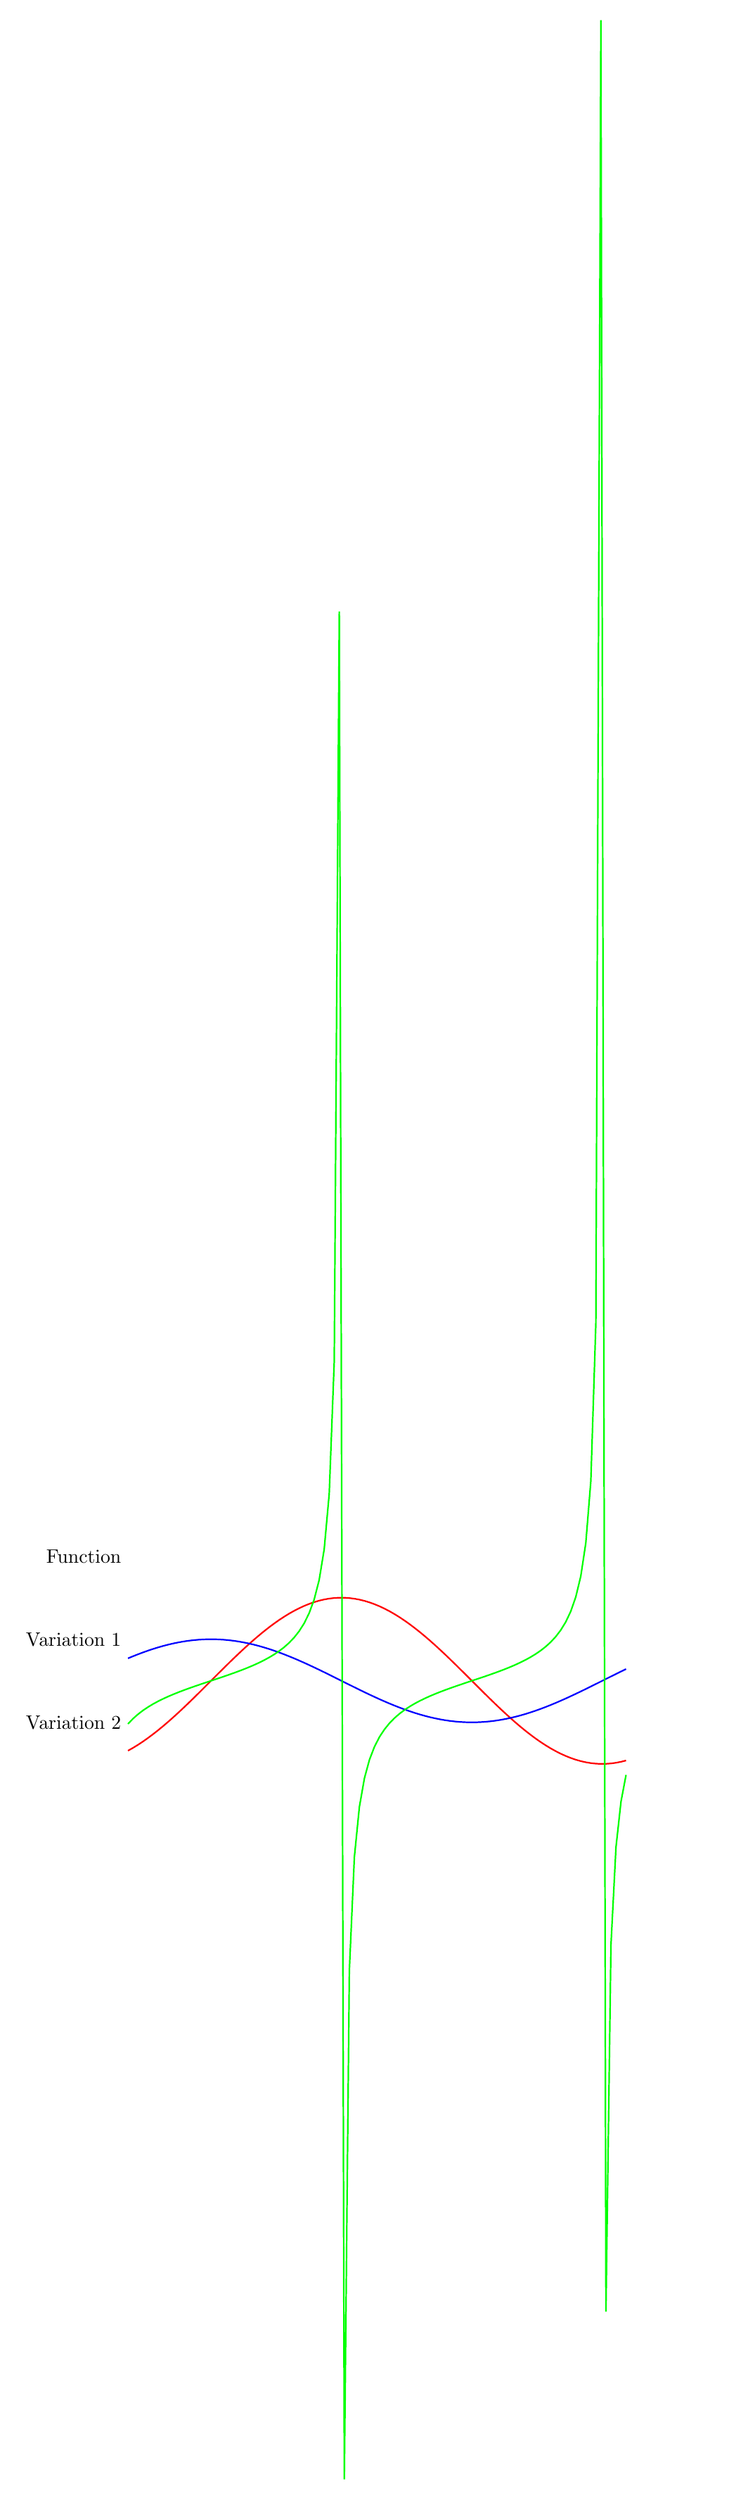
\begin{tikzpicture}[scale=1.5]

% Whiteboard background
\fill[white] (0,-2) rectangle (6,4);

% Red curve representing the main function
\draw[red, thick] plot[domain=-1:5,samples=100] (\x,{sin(\x r)}); % Example function

% Blue curve representing a variation or aspect of the function
\draw[blue, thick] plot[domain=-1:5,samples=100] (\x,{cos(\x r)/2}); % Example variation

% Green curve representing another variation or aspect of the function
\draw[green, thick] plot[domain=-1:5,samples=100] (\x,{tan(\x r)/3}); % Example variation

% Labels for clarity
\node at (-1, 1.5) [left] {Function};
\node at (-1, 0.5) [left] {Variation 1};
\node at (-1, -0.5) [left] {Variation 2};

\end{tikzpicture}

\end{document}